% TODO: Explicar en qué patrones de fraudes estamos interesados
\subsection{Fraud pattern detection}

In the following the target fraud patterns to be detected are described. In addition, some others patterns that could also be potentially detected are also commented.

\begin{comment}
TODO: Comentar sobre la naturaleza del sistema que estamos diseñando
-------------------------
El sistema que estamos diseñando es orientado a detección y alerta de fraude sobre transacciones YA REALIZADAS!

NO sobre intentos de transacciones! (preventivo)

Se podría escalar a ello para evitar la realización de transacciones que fuesen detectadas como posibles fraudes, sin embargo esto complicaría la gestión de los filtros ya que:

1. filtro detectaría posible fraude; transacción tentativa quedaría en espera
2. filtro tendría que recibir de vuelta del sistema bancario si al final se autorizó, a pesar de la alerta, esa transacción o no, para poder eliminarla / limpiar el filtro.
Si esto no sucediera así entonces en el caso de que no se autorizara finalmente la transacción tentativa podríamos estar teniendo en el filtro una "falsa transacción" y por tanto estar causando conflictos o generando nuevas alertas que no deberían de estar generándose por culpa de no haber limpiado el filtro de esta transacción no realizada.
-------------------------
\end{comment}

\subsubsection{Are there two or more withdrawals with the same card at ATMs from different locations (at the same time)?}\label{fraud-pattern-1}



The pattern describes the situation in which two or more withdrawals with the same card at ATMs from different locations are registered, so that the distance between the locations of the two ATMs can not be physically covered in the difference in time between the two withdrawals.

\begin{figure}[H]
    \centering
    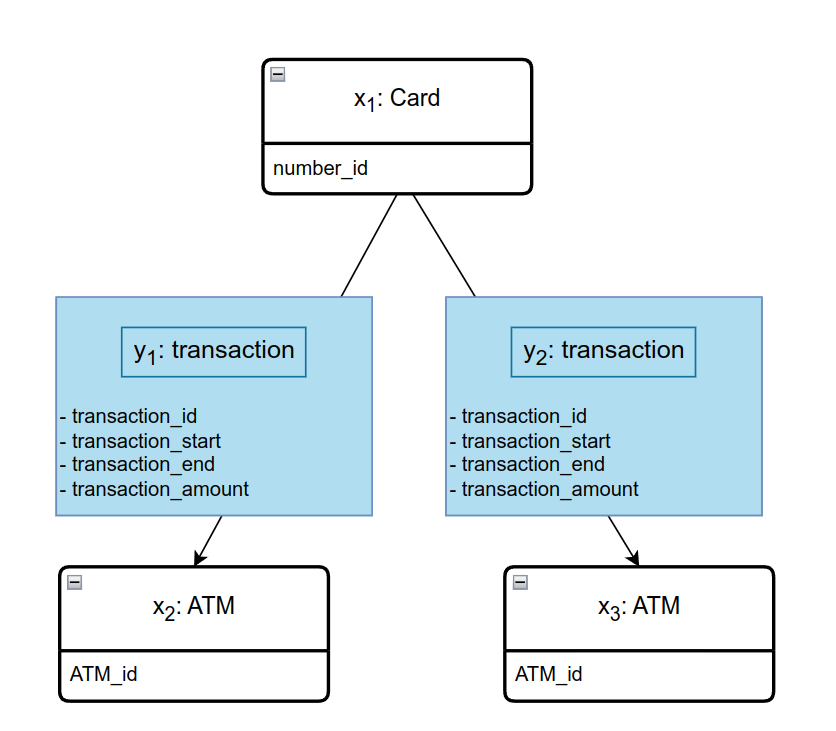
\includegraphics[scale = 0.35]{images/Frauds/fraud-pattern-1.png}
    \caption{Fraud pattern 1}
    \label{img:fraud-pattern-1}
\end{figure}

The pattern graph shape is represented in Figure \ref{img:fraud-pattern-1}, which can be formally described as:
$$
x2.id \ne x3.id 
$$
$$\land$$
$$
\text{y2.transaction\_start} - \text{y1.transaction\_end} < T_{min}(x2.location, x3.location)
$$
where location represents the GPS coordinates of the corresponding ATM, that is, for example: $x2.location = (x2.loc\_latitude, x2.loc\_longitude)$.

\begin{comment}
$$
\small
x2.id \ne x3.id \ \land \ \text{y2.transaction\_start} - \text{y1.transaction\_end} < T_{min}(x2.location, x3.location)
$$
\end{comment}

An example of this kind of anomalous card-ATM interaction, could be one in which a withdrawal with a certain card is finished at time 22:14 in Barcelona, and then another withdrawal with that same card starts at time 22:56 of that same day in Madrid. Clearly this should be reported as a this kind of pattern since it is impossible, for the time being, to cover the distance between these two cities in that time difference.

% TODO: Mostrar ejemplo con el timeline del pipeline de eventos transacción...


\subsubsection{Other patterns...}
Other possible ideas:

% TODO: Describir estos patrones
- Patrón del "paraguas": muchas transacciones seguidas (generalmente de pequeño tamaño), en el mismo o en distintos ATMs -> % TODO: Encontrar referencias / artículos donde se comenten y expliquen más estos tipos de fraudes.

- ATM of the client does not match an ATM close to a certain distance to the client registered address.
Transaction located in an ATM out of the threshold distance of the usual / registered address of the client.